\documentclass[8pt,landscape,a4paper]{article}
\usepackage[utf8]{inputenc}
\usepackage[ngerman]{babel}
\usepackage[T1]{fontenc}
%\usepackage[LY1,T1]{fontenc}
%\usepackage{frutigernext}
%\usepackage[lf,minionint]{MinionPro}
\usepackage{tikz}
\usetikzlibrary{shapes,positioning,arrows,fit,calc,graphs,graphs.standard}
\usepackage[nosf]{kpfonts}
\usepackage[t1]{sourcesanspro}
\usepackage{multicol}
\usepackage{wrapfig}
\usepackage[top=0mm,bottom=1mm,left=0mm,right=1mm]{geometry}
\usepackage[framemethod=tikz]{mdframed}
\usepackage{microtype}
\usepackage{pdfpages}
\usepackage{graphicx}
\usepackage{lipsum}  % generates filler text
\usepackage{xcolor}
\usepackage{listings}
\usepackage{xparse}
\usepackage{courier} %% Sets font for listing as Courier.
\usepackage{CJKutf8}


\let\bar\overline

\definecolor{myblue}{cmyk}{1,.72,0,.38}
\definecolor{orange}{rgb}{1,0.5,0}
\definecolor{mynicegreen}{RGB}{5,255,102}

\def\firstcircle{(0,0) circle (1.5cm)}
\def\secondcircle{(0:2cm) circle (1.5cm)}

\colorlet{circle edge}{myblue}
\colorlet{circle area}{myblue!5}

\tikzset{filled/.style={fill=circle area, draw=circle edge, thick},
    outline/.style={draw=circle edge, thick}}
    
\pgfdeclarelayer{background}
\pgfsetlayers{background,main}

\everymath\expandafter{\the\everymath \color{myblue}}
\everydisplay\expandafter{\the\everydisplay \color{myblue}}

\renewcommand{\baselinestretch}{.8}
\pagestyle{empty}

% \global\mdfdefinestyle{header}{%
% linecolor=gray,linewidth=1pt,%
% leftmargin=0mm,rightmargin=0mm,skipbelow=0mm,skipabove=0mm,
% }

% \newcommand{\header}{
% \begin{mdframed}[style=header]
% \footnotesize
% \sffamily
% Hilfszettel zur Klausur\\
% von~Jigao,~Seite~\thepage~von~2
% \end{mdframed}
% }

\makeatletter % Author: https://tex.stackexchange.com/questions/218587/how-to-set-one-header-for-each-page-using-multicols
\renewcommand{\section}{\@startsection{section}{1}{0mm}%
                                {0ex}%
                                {.1ex}%x
                                {\color{myblue}\sffamily\small\bfseries}}
% \renewcommand{\subsection}{\@startsection{subsection}{1}{0mm}%
%                                 {0ex}%
%                                 {.1ex}%x
%                                 {\color{myblue}\sffamily\bfseries}}
\newcommand{\rtext}[1]{\textcolor{red}{\textbf{#1}}}
\newcommand{\redtext}[1]{\textcolor{red}{#1}}
\newcommand{\btext}[1]{\textcolor{blue}{\textbf{#1}}}
\newcommand{\bluetext}[1]{\textcolor{blue}{#1}}
\newcommand{\orangetext}[1]{\textcolor{orange}{#1}}
\newcommand{\greentext}[1]{\textcolor{mynicegreen}{#1}}
\newcommand{\mysubsection}[1]{\textcolor{myblue}{\scriptsize{\textbf{#1}}}}
\newcommand{\hlc}[2][yellow]{{%
    \colorlet{foo}{#1}%
    \sethlcolor{foo}\hl{#2}}%
}
\newcommand{\hlgray}[1]{%
  \hlc[lightgray!40]{#1}
}

% \def\multi@column@out{%
%    \ifnum\outputpenalty <-\@M
%    \speci@ls \else
%    \ifvoid\colbreak@box\else
%      \mult@info\@ne{Re-adding forced
%                break(s) for splitting}%
%      \setbox\@cclv\vbox{%
%         \unvbox\colbreak@box
%         \penalty-\@Mv\unvbox\@cclv}%
%    \fi
%    \splittopskip\topskip
%    \splitmaxdepth\maxdepth
%    \dimen@\@colroom
%    \divide\skip\footins\col@number
%    \ifvoid\footins \else
%       \leave@mult@footins
%    \fi
%    \let\ifshr@kingsaved\ifshr@king
%    \ifvbox \@kludgeins
%      \advance \dimen@ -\ht\@kludgeins
%      \ifdim \wd\@kludgeins>\z@
%         \shr@nkingtrue
%      \fi
%    \fi
%    \process@cols\mult@gfirstbox{%
% %%%%% START CHANGE
% \ifnum
% \count@=\numexpr\mult@rightbox+2\relax
%           \setbox\count@\vsplit\@cclv to \dimexpr \dimen@-1cm\relax
% % \setbox\count@\vbox to \dimen@{\vbox to 1cm{\header}\unvbox\count@\vss}%
% \else
%       \setbox\count@\vsplit\@cclv to \dimen@
% \fi
% %%%%% END CHANGE
%             \set@keptmarks
%             \setbox\count@
%                  \vbox to\dimen@
%                   {\unvbox\count@
%                    \remove@discardable@items
%                    \ifshr@nking\vfill\fi}%
%            }%
%    \setbox\mult@rightbox
%        \vsplit\@cclv to\dimen@
%    \set@keptmarks
%    \setbox\mult@rightbox\vbox to\dimen@
%           {\unvbox\mult@rightbox
%            \remove@discardable@items
%            \ifshr@nking\vfill\fi}%
%    \let\ifshr@king\ifshr@kingsaved
%    \ifvoid\@cclv \else
%        \unvbox\@cclv
%        \ifnum\outputpenalty=\@M
%        \else
%           \penalty\outputpenalty
%        \fi
%        \ifvoid\footins\else
%          \PackageWarning{multicol}%
%           {I moved some lines to
%            the next page.\MessageBreak
%            Footnotes on page
%            \thepage\space might be wrong}%
%        \fi
%        \ifnum \c@tracingmulticols>\thr@@
%                     \hrule\allowbreak \fi
%    \fi
%    \ifx\@empty\kept@firstmark
%       \let\firstmark\kept@topmark
%       \let\botmark\kept@topmark
%    \else
%       \let\firstmark\kept@firstmark
%       \let\botmark\kept@botmark
%    \fi
%    \let\topmark\kept@topmark
%    \mult@info\tw@
%         {Use kept top mark:\MessageBreak
%           \meaning\kept@topmark
%          \MessageBreak
%          Use kept first mark:\MessageBreak
%           \meaning\kept@firstmark
%         \MessageBreak
%          Use kept bot mark:\MessageBreak
%           \meaning\kept@botmark
%         \MessageBreak
%          Produce first mark:\MessageBreak
%           \meaning\firstmark
%         \MessageBreak
%         Produce bot mark:\MessageBreak
%           \meaning\botmark
%          \@gobbletwo}%
%    \setbox\@cclv\vbox{\unvbox\partial@page
%                       \page@sofar}%
%    \@makecol\@outputpage
%      \global\let\kept@topmark\botmark
%      \global\let\kept@firstmark\@empty
%      \global\let\kept@botmark\@empty
%      \mult@info\tw@
%         {(Re)Init top mark:\MessageBreak
%          \meaning\kept@topmark
%          \@gobbletwo}%
%    \global\@colroom\@colht
%    \global \@mparbottom \z@
%    \process@deferreds
%    \@whilesw\if@fcolmade\fi{\@outputpage
%       \global\@colroom\@colht
%       \process@deferreds}%
%    \mult@info\@ne
%      {Colroom:\MessageBreak
%       \the\@colht\space
%               after float space removed
%               = \the\@colroom \@gobble}%
%     \set@mult@vsize \global
%   \fi}

\makeatother
\setlength{\parindent}{0pt}

\NewDocumentCommand{\codeword}{v}{%
\texttt{\textcolor{blue}{#1}}%
}

% \lstset{language=Java, breakatwhitespace=true, keywordstyle={\bfseries \color{blue}}}

\lstset{
  language=Java,
  tabsize = 2, %% Sets tab space width.
  showstringspaces = false, %% Prevents space marking in strings, string is defined as the text that is generally printed directly to the console.
  numbers = left, %% Displays line numbers on the left.
  commentstyle = {\bfseries \color{green}}, %% Sets comment color.
  keywordstyle = {\bfseries \color{blue}}, %% Sets  keyword color.
  stringstyle = {\bfseries \color{red}}, %% Sets  string color.
  rulecolor = {\bfseries \color{black}}, %% Sets frame color to avoid being affected by text color.
  basicstyle = \tiny \ttfamily , %% Sets listing font and size.
  breaklines = true, %% Enables line breaking.
  numberstyle = \tiny,
}

\begin{document}
%\footnotesize
\tiny
\begin{multicols*}{6}
\section{Introduction}
\redtext{Enterprise SY architecture:}Cs, Web S, APP Ss, MsgQueue, Pub/Sub SY, DBs 
\\ 
\redtext{Distributed APP} developed on \bluetext{sockets}.
(Fallacies,
Interoperability in spite of heterogeneity,
Data representation and encoding,
Parameter passing convention calling remote procedures,
Atomic execution of TX,
Enable APP integration,
Data persistence)
\\
\redtext{Middleware} as layer between \bluetext{transport \& application layer}
or \bluetext{Above OS and below APP}. 
comprises \bluetext{services and abstractions}(RMI, Messaging, PubSub,TX,Naming) that facilitate the
design, development, and deployment of distributed APP in
\bluetext{heterogeneous, networked environments}.
Deals with interoperability
\begin{CJK*}{UTF8}{gbsn}
\bluetext{互通性}
\end{CJK*}, SY integration
\textbar 
C request/response $\leftrightarrow$ Middleware $\leftrightarrow$ S. 
\textbar
All Computers \bluetext{share single distributed APP and Middleware.}
\\
\redtext{Heterogeneity}:
Computer architecture(big, little endian), 
OS(Comm. sub-system), 
Host and network representation of data, 
Programming language(Representation of characters)
\\
\redtext{Ilities:}
Reliable; 
Fault-tolerant; 
Highly available; 
Recoverable; 
Consistent; 
Scalable; 
Predictable pref.; 
Secure; 
Heterogeneous; 
Open
% \\
% \rtext{8 Fallacies}
% \rtext{1.Network Reliable} 
% \bluetext{Assumptions:}Power Supply, Hard Disk, Node Failures, Config., Bugs
% \bluetext{Effect:}APP hangs, crashes 
% \bluetext{Countermeasures:}
% Redundancy HW\&SW systems,middleware \&application; 
% Catch Exceptions; 
% Check Codes, React; 
% Retry After Timeouts;
% pos. neg. ACK; 
% Identify \& ignore duplicates; 
% idempotent operations
% \rtext{2.Latency\begin{CJK*}{UTF8}{gbsn}延迟\end{CJK*} Is Zero}
% time For Data Transfer(speed Of Light); 
% Bandwidth:how Much Data transferred (bit/s)
% \textbar
% Local Call: Push and a Jump to Subroutine;
% SY Call: OS, 100s of assembly;
% Call across LAN: SY calls on caller $+$ callee $+$ network latency;
% Call across WAN: transmission delay
% \redtext{3.Bandwidth is infinite.
% 4.The network is secure.
% 5.Topology doesn't change.
% 6.There is one administrator.
% 7.Transport cost is zero.
% 8.The network is homogeneous}
% \\
% \bluetext{Standardization}:
% Official:ISO, ITU, DIN, Semi-official: IEEE, W3C, OpenGroup
\section{Comm. Basics}
\redtext{ISO OSI:}
Open Systems Interconnection model, 
Basis for standards development on SY interconnection,
Reference model.
\textbar
\redtext{Layers:}
\bluetext{
Application(Peer protocol: HTTP, DNS, FTP);
Presentation;
Session;
Transport: TCP/UDP;
Network: IP;
Data link;
Physical}
\\ 
\redtext{IPv4 v6(no checksum):}
Relays datagrams accross networks,
Routing enables internetworking,
Deliver packet from source to host address,
Foundation for TCP/UDP
\\
\redtext{IP routing:}routing protocol,
\bluetext{BGP} used in internet:
Border Gateway Protocol,
Routing between AS (Autonomous systems, provider or bigger organization),
Exchanges routing and reachability information between AS.
\\
\redtext{TCP:} for \bluetext{HTTP, RPC},
Slower than UDP, but with reliability using ACK,
Connection oriented protocol, session is initiated,
Provides ordering, sequencing,
Flow control, sender can't overflow receiver(same speed sending, receiving),
PortNum in TCP protocol(not in IP protocol)
\\
\redtext{UDP:} for \bluetext{DNS, Video, Voice},
Faster than TCP,
Connectionless(no session);
Best-effort;
Packet independent; 
No guaranteed delivery;
No ordering guarantees;
P2P and P2-multipoint.
\\
\redtext{Ports:}
a 16 bit number to local host to identify the connection, 
to differentiate APPs, if packet arrive;
Separate for \bluetext{UDP and TCP};
$0-1023$ reserved to root,
$1024 - 65535$  available to regular user;
http 80/tcp, ftp 21/tcp, ssh 22/tcp, telnet 23/tcp, finger 79/tcp, snmp 161/udp
\\
\redtext{APP Layer protocol:}
Set of rules specifying data transfer
between computing end-points
(Connection establishment \& tear-down
Data representation,
Comm);
\bluetext{DHCP} (Dynamic Host Configuration Protocol),
\bluetext{HTTP} (Hypertext Transfer Protocol),
\bluetext{FTP} (File Transfer Protocol),
\bluetext{Telnet} (Telnet Remote Protocol),
\bluetext{SSH} (Secure Shell Remote Protocol),
\bluetext{SIP} (Session Initiation Protocol),
\bluetext{POP3} (Post Office Protocol 3),
\bluetext{SMTP} (Simple Mail Transfer Protocol),
\bluetext{IMAP} (Internet Message Access Protocol),
\textbar \textbar
browser retreives web page(HTTP 1.1 over TCP, HTTP, FTP, SMTP)
\\
\redtext{HTTP/1.0 C S:}
\bluetext{Request}: GET <path>/index.html HTTP/1.0
\bluetext{Response}: HTTP/1.0 200 OK
\bluetext{ErrorResponse}: HTTP/1.0 404 Not Found 
\textbar \textbar
\redtext{HTTP/1.1:}
HyperText Transfer Protocol,
Request/Response protocol for C S comm. on top of TCP
(Browser,
RESTFUL API‘s,
SOAP over HTTP,
NoSQL databases)
\bluetext{Methods:}
\bluetext{GET:}cacheable get info by Request-URI
\bluetext{HEAD:} like GET but MUST NOT return a message-body
\bluetext{POST:} post a form (bulletin board), uploading data,
can be a data-accepting process
Responses not cacheable(200 (OK), 204(No Content), 201
(Created), 303 (See Other)) 
\bluetext{PUT:} Enclosed entity to be stored under Request-URI
Responses not cacheable
\bluetext{DELETE:} Delete the resource by Request-URI
Response: 200 (OK), 202 (Accepted), 204 (No Content)
\bluetext{TRACE:} for diagnostics
\bluetext{CONNECT:} to initialize secure connection, HTTPS on port 443,
Proxy is asked to forward the TCP connection
\textbar
\redtext{HTTP/1.1 proxy:}C \bluetext{GET req.} $\rightarrow$ Proxy, but not in cache. 
Proxy \bluetext{GET req.} $\rightarrow$ Origin, Origin $\rightarrow$ Proxy response.
C \bluetext{GET req.} $\rightarrow$ Proxy, Proxy $\rightarrow$ C cached resp.
\textbar
\redtext{HTTP/2.0:}
Better utilization network capacity,
Headers compressed,
On a single connection req and resp interleaved,
Prioritization of requests
% FIXME: can be removed
\textbar \textbar \textbar
GET/HTTP/1.1
Host:www.tum.de
Connection:keep-alive
Accept: text/html,application/xhtml+xml,application/xml;q=0.9, image/webp, */*;q=0.8
User-Agent: Mozilla/5.0 (X11; Linux x86\_64) AppleWebKit/537.36 (KHTML, like Gecko) Chrome/37.0.2062.120 Safari/537.36
Accept-Encoding: gzip,deflate,sdch
\textbar \textbar \textbar
HTTP/1.1 200 OK
Date: Wed, 08 Oct 2014 15:25:53 GMT
Server: Apache
X-Powered-By: PHP/5.5.17
Content-Encoding: gzip
%
%
%
\\
\mysubsection{Socket}
\\
Move data/Msg/(invoke operation/service and return result/failure) 
from APP I on Host A to APP K on Host B.
\redtext{Client}:Issues req to S(send \& receive).
\redtext{Server}:Starts up and listens for connections, req.s, and sends/receives.
\redtext{C S eg.}: \bluetext{P2P} telnet/telnetd, ftp/ftpd (sftp/sftpd), Firefox/Apache.
\\
\rtext{Socket}: using network API, network programming abstraction for comm. among processes (APPs) based on (Unix) file
descriptors.
\bluetext{File/Socket descriptor}:int for open file managed by the OS, 
In \orangetext{Unix any I/O} by reading/writing from/to file descriptors.
\textbar
\redtext{Socket types}: 
\bluetext{Stream socket:}telent, HTTP, browser, java.net.ServerSocket, TCP based(Ordering guaranteed, Error-free); 
\bluetext{Datagram socket:}java.net.DatagramSocket, UDP based; 
\bluetext{IPv4\&IPv6}
\\
\redtext{2 end-points determine a connection}: IP address (host address)$+$Port number
\\
\rtext{SetUp,UseSockets}
\orangetext{S Create:}
\lstinline{final ServerSocket ss = new;/*localhost only*/ ss.bind(new InetSocketAddress("0.0.0.0", port)); while (true) {Socket clientSocket = ss.accept();/*Block till C*/}
\orangetext{C connect S:}
\lstinline{Socket s = new; s.connect(new InetSocketAddress("127.0.0.1", port)); PrintWriter output = new PW(s.getOutputStream()); BufferedReader input = new BR(new InputStreamReader(s.getInputStream())); output.write(req + "\r\n");/*to S*/ output.flush();}
\orangetext{S handle req.:}
\lstinline{/*in while true*/ BufferedReader in = new BR(new InputStreamReader(clientSocket.getInputStream(), Constants.TELNET_ENCODING)); PrintWriter out = new PW(new OutputStreamWriter(clientSocket.getOutputStream(), Constants.TELNET_ENCODING)); String firstLine; while ((firstLine = in.readLine()) != null) /*req from C*/ String res = kv.process(firstLine); out.write(res); /*to C*/ out.flush();}
\orangetext{C read resp.:}
\lstinline{/*after C connect S*/String response = input.readline(); s.close();}
\orangetext{S shutdown:}
\lstinline{ss.close();}
\adjincludegraphics[width=1\linewidth, trim={0 0 0 {.12\height}},clip]{chap1_1.png}
\redtext{\hlgray{Finite state machines FSM}} \hlgray{describing} 
\redtext{\hlgray{a comm. session C S}}.
\hlgray{C\&S keep comm. session open and exchange Msg until one of them closed.}
\orangetext{\hlgray{accept:}} \hlgray{a} \lstinline{while loop}:
\orangetext{\hlgray{create a new socket (and th.) for commu. with C}}
\\
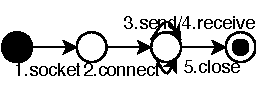
\includegraphics[width=.49\linewidth]{client_FSM.pdf}
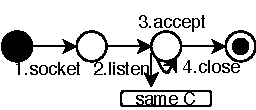
\includegraphics[width=.49\linewidth]{server_FSM.pdf}
\rtext{K V Server:} C get, set Table in S: 
\bluetext{PUT tablename key value\textbackslash r\textbackslash n}, 
\bluetext{GET tablename key}
\textbar
\redtext{C:}
\orangetext{C.java:}
\lstinline{KVTable<AssessmentInformation> kvc = new KVTable<~>(); kvc.put("middleware", new AssessmentInformation(1.3);}
\orangetext{KVTable.java in put():}
\lstinline{String jsonStr = gs.toJson(value); String enc_value = encodeBase64(jsonStr); this.activeConnection.write("PUT " + this.table + " " + key + " " + enc_value + "\r\n");}
\orangetext{ActiveConnection.java in write():}
\lstinline{PrintWriter output...; output.write(..); output.flush();}
\redtext{S:}
\orangetext{ConnectionHandleThread.java}
\lstinline{BufferedReader in = new BufferedReader(new ISReader(clientSocket.getIS(),...)); String line = in.readLine();}
\orangetext{KVStore.java}
\lstinline{StringTokenizer st = new StringTokenizer(firstLine, " \r\n"); String command = st.nextToken(); if (command == "GET")/*GET PUT else*/}
\orangetext{ConnectionHandleThread.java}
\lstinline{PrintWriter out = new PrintWriter(new OutputStreamWriter(clientSocket.getOutputStream(),...)); out.write(res);/*to C*/ out.flush();}
\\
\mysubsection{NIO(NonblockingSockets),multi.threaded}
\\
\redtext{Synchronous}: 
Single th. read data from C(stream) and blocked until done
\rtext{Asynchronous}: 
th. $\rightarrow$ \bluetext{Channel}: 
read data into \bluetext{Buffer}; 
\bluetext{Channel} $\rightarrow$ \bluetext{Buffer}: 
fill data into \bluetext{Buffer}; 
Th. $\rightarrow$ \bluetext{Buffer}: 
check data in \bluetext{Buffer} (main th. not blocked)
\\
\rtext{\hlgray{Syn. vs. Asyn.}}: 
\bluetext{Syn}: Th. acts and waits until \orangetext{Syn. I/O} done; 
\orangetext{}text{Limited scalability}, a th. per I/O connection
(Overhead:\orangetext{context switching} $\rightarrow$ time between diff. tasks)
\bluetext{Asyn}: Pass req. to OS-kernel and do other tasks 
$\rightarrow$\orangetext{worker th.}\lstinline{while(true)} 
\rtext{++:}
\orangetext{\hlgray{only Compute, never Blocked, no Context Swtich, Asyn. I/O}}
\hlgray{
Scalability, 
Consumers not block S long time,
One th. handle multi. sockets
}
\rtext{--:}
\hlgray{
Complex handling code,
Requires different kind of architecture(Eventloops)
}
\\
\rtext{Java NIO Channels}: 
All \orangetext{I/O operations} done with \bluetext{channels(File, TCP, UDP)};
Multi types of \bluetext{channels}
(FileChannel(File on disk), 
DatagramChannel (UDP), 
SocketChannel (TCP, support concurrent read/write), 
ServerSocketChannel (TCP));
Responsibility(\orangetext{Read, write buffer})
\\
\rtext{\hlgray{Sequence Dia multi th:}}
\btext{\hlgray{n times C and Th.}}
\textbar
\bluetext{\hlgray{Ci to S:}} \hlgray{connect}, 
\bluetext{\hlgray{S to Th.i}}, 
\bluetext{\hlgray{Ci to S to Th.i:}} \hlgray{getTime()},
\bluetext{\hlgray{Th.i to S to C:}} \hlgray{20:00}
\\
\rtext{\hlgray{S Create:}} 
\hlgray{same as single th. above}
\orangetext{\hlgray{S Create}}
\bluetext{\hlgray{instead of block IO in while:}}
\lstinline{HandleRequest hr = new HandleRequest(client); hr.start();}
\\
\rtext{\hlgray{HandleRequest as Th.:}}
\lstinline{class HandleRequest extends Thread{private Socket c;HandleRequest(Socket c){c = c;/*]*/run(){String msg = c.receive()if(msg == "getTime"){String res = getTime();c.send(res);c.close();}
\\
\rtext{\hlgray{C:}}
\lstinline{class Client{public void sendMessage(){String ip'112.32.86.113'; int port = 8883; String msg = "getTime"; Socket c = new Socket(); c.connect(ip, port); c.send(msg); String res = client.receive(); client.close(); print res;}
\\
\rtext{\hlgray{Sequence Dia single th:}}
\btext{\hlgray{n times C}}
\textbar
\bluetext{\hlgray{Ci to S:}} \hlgray{connect}, 
\bluetext{\hlgray{Ci to S to Th.i:}} \hlgray{getTime()},
\hlgray{all C sent, S start with Zeitraum to process n req.}
\bluetext{\hlgray{Th.i to S to C:}} \hlgray{20:00 resp. same order as sent req.}
\\
\redtext{\hlgray{Selector:}} 
\hlgray{select multi asyn. Channels to match a EventLoop}
\orangetext{\hlgray{Setup channel:}}
\lstinline{Hashmap<SocketChannel, byte[]> pendingData; ServerSocketChannel ssc = new SSC(); ssc.connect("127.0.0.1", 8883); Selector selector = new Selector(); ssc.register(selector, SelectionKey.ACCEPT);}
\rtext{OR}
\lstinline{ServerSocketChannel ssC = SSC.open();ssC.configureBlocking(false);InetSocketAddress isa  = new ISA(InetAddress.getByName("localhost"), 5559);ssC.socket().bind(isa);}
\orangetext{\hlgray{handleRequest():}}
\lstinline{public byte[] handleRequest(byte[] input){return Bytes.toBytes(System.nanoTime());}
\orangetext{\hlgray{Eventloop:}}
\lstinline{public void start() throws IOException {while (true) try {selector.select();/*get List*/ Iterator selectedKeys = selector.selectedKeys().iterator(); while (selectedKeys.hasNext()) {SelectionKey key = (SelectionKey) selectedKeys.next(); selectedKeys.remove(); if (key.isAcceptable()) {ServerSocketChannel channel = (SSC)key.channel(); SocketChannel sC = channel.accept(); sC.configureBlocking(false); sC.register(this.selector, SelectionKey.READ);/*wake up when sth to read*/ else if (key.isReadable()) {SocketChannel channel = (SC)key.channel(); byte[] res = handleRequest(channel.read()); pendingData.add(channel, res); key.interesOps(SelectionKey.WRITE); else if (key.isWritable()) {SocketChannel channel = (SC)key.channel(); data = pendingData.get(channel); if(data == (byte[])"getTime"){channel.write((byte[])getTime()); key.interestOps(SelectionKey.READ); catch (e) {e.printStackTrace();}
% \orangetext{Register selector:}
% \lstinline{Selector s = SelectorProvider.provider().openSelector(); serverChannel.register(s, SelectionKey.OP_ACCEPT); private void accept(SelectionKey key) throws IOException {ServerSocketChannel sSC = (SSC) key.channel(); SocketChannel sC = sSC.accept(); sC.configureBlocking(false); sC.register(this.s, SelectionKey.OP_READ);/*wake up when sth to read*/}
\orangetext{Read:}
\lstinline{private void read(SelectionKey key) throws IOException {SocketChannel sC = (SC) key.channel(); this.readBuffer.clear(); int numRead = sC.read(this.readBuffer);/*in Buffer*/ if (numRead == -1) { key.channel().close(); key.cancel(); return;/*]*/byte[] dataCopy = new byte[numRead]; arraycopy(this.readBuffer.array(), 0, dataCopy, 0, numRead); handleRequest(sC, dataCopy);}
\orangetext{Write:}
\lstinline{private void write(SelectionKey key) throws IOException { SocketChannel sC = (SC) key.channel(); List queue = (List) this.pendingData.get(sC); while (!queue.isEmpty()) { ByteBuffer buf = (ByteBuffer) queue.get(0); socketChannel.write(buf); if (buf.remaining() > 0) {break;/*]*/queue.remove(0);/*]*/ if (queue.isEmpty()) {key.interestOps(SelectionKey.OP\_READ);/*]*/}
\\
\redtext{\hlgray{Protocol Design:}}
\hlgray{complex number as string: c = (a, b, n)}, 
$n \in {s,p}$,
$op \in \{add, sub, mul, div, poloar\}$,
\orangetext{\hlgray{C to S req.:}}\hlgray{m<c1;c2;op>, 
<(1.0,1.0,s);(2.0,4.0,s);add>
Status:} $st\in\{OK,msgIncomplete.msgFormatError,serverError\}$,
\orangetext{\hlgray{S to C resp.:}}
\hlgray{m2<Cr; st>, 
<(3.0,5.0,s); ok>}
\textbar
\redtext{\hlgray{Sequence Dia.:}}
\hlgray{C2S: m1<(a1,b1);(a2,b2);".add">} 
\redtext{+}
\hlgray{S2C:m2<(a1+a2,b1+b2);".ok">;
C2S: m1<(a1,b1);(a}
\redtext{+}
\hlgray{m2<(0.0,0.0);"msgIncomplete">}
\orangetext{\hlgray{execution error, processing correct}}
\section{C2 EXTERNAL DATA REPRESENTATION, Presentation Layer} 
\rtext{Heterogeneity}
HW: Diff. HW architectures store bytes:Big, Small Endian
ProgrammingLanguage:Diff. PL store data types differently:AB, 0AB
\rtext{Transformation between representations}: Transformation between local and remote representations|Information may lost
\textbf{Two realizations}:
$1.$\textbf{Pairwise transformation between $n$ local representations}(vollständigGraph,$\#n^2 - n$, Either sender or receiver has to transform) 
$2.$\textbf{Transformation to and from canonical representation}(a single canonical $C$ as intermediate representation|No local information about communication
partner needed| $\#2*(n-2)$, $ -2$if canonical is one of $n$)
\rtext{XDR} partOf NFS, OSPresentationLayer, encodes only data items, no meta information about their types +:easy, -:Receiver lost data description
\textbar exactly 32 bit integer is stored according to \textbf{big endian} +:Fixed length reduces computation. -:wasting
\textbar Data is encoded into blocks of multiples of 4: n-bytes contain data; r-bytes are used for padding with n + r mod 4 = 0
\textbar int: int32; float=Sign+Exponent+Mantissa, String=length\_int32+bytes, array=length\_int32+ele
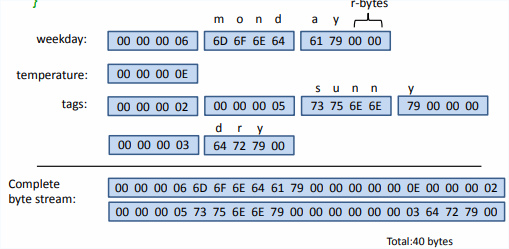
\includegraphics[width=.8\linewidth]{chap2_2.png} 
\lstinline{struct forecast:String weekday;int temperature;String tags<>;}
\rtext{ASN.1}:Abstract description of data types,telecommunication,internet protocol 
\textbar Enables exchange in heterogeneous systems
\textbar \btext{abstractSyntax $\overset{compiler}{\rightarrow}$ concreteSyntax Java, C++, they transfer syntax using encodingRules}
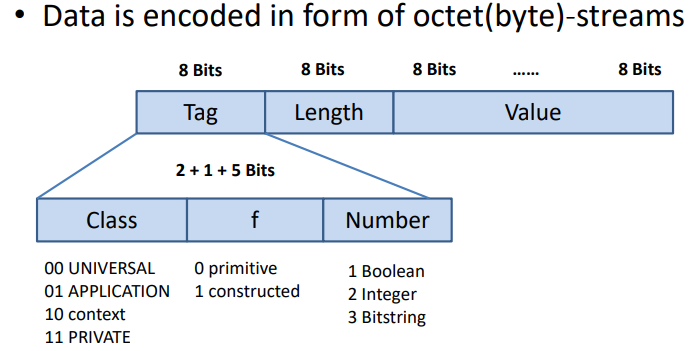
\includegraphics[width=.45\linewidth]{chap2_3.png}
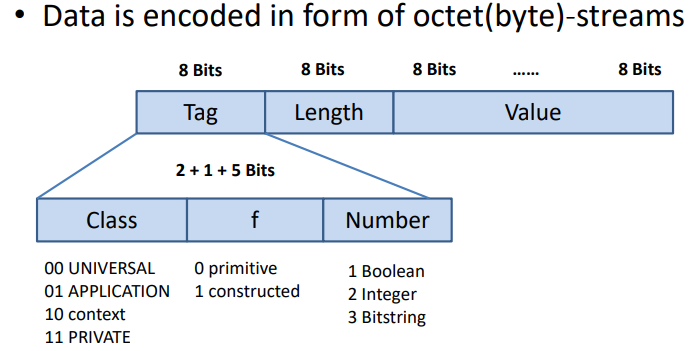
\includegraphics[width=.45\linewidth]{chap2_4.png}
\lstinline{Forecast::==SET{weekday IA5String,temperature Interger,tags SEQUENCE OF IS5String;}
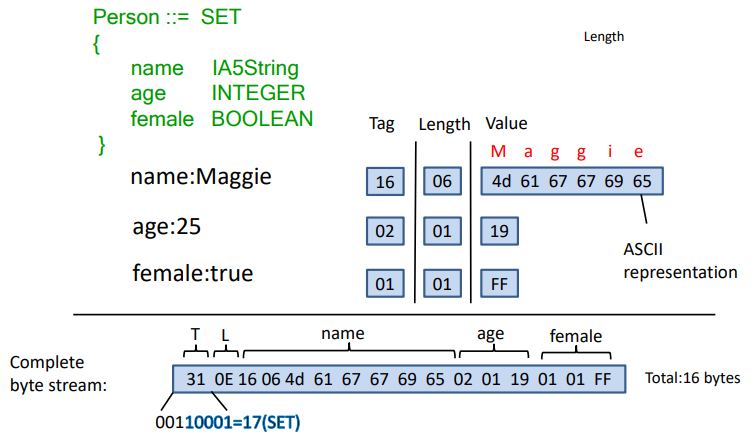
\includegraphics[width=.45\linewidth]{chap2_5.png}
\textbar encodes type information, +:receiver not need to know data description,-:additional overhead
\rtext{Java object serialization,JOS}
Stream-based transmission of serialized objects(Via TCP or UDP sockets)
, Receiver of object needs implementation of class
, Serialization does not require class specific code(Java reflection)
, Class implements java.io.Serializable interface
\textbf{-}: locked into Java(No support for heterogeneous systems), No support for versioning(If the serialized class changes, all network nodes
have to be updated)
\rtext{serialize:obj2bit}\lstinline{Socket s = new Socket("localhost", 8022);ObjectOutputStream oos = new ObjectOutputStream(s.getOutputStream()); oos.writeObject(obj);}
\rtext{deserialize:bit2obj}\lstinline{ServerSocket ss = new ServerSocket(8022);Socket s = serverSocket.accept();ObjectInputStream ois = new ObjectInputStream(s.getInputStream());obj=(Obj)ois.readObject();}
\rtext{XML}De facto standard for data exchange
\textbar Schema: \lstinline{<xsd:element name="forecast"> <xsd:complexType> <xsd:all> <xsd:element name="weekday" type="xsd:string"/> <xsd:element name="temperature" type="xsd:integer"/> <xsd:element name="tags">
<xsd:complexType> <xsd:sequence> <xsd:element name="tag" type="xsd:string" maxOccurs=\"unbounded\"/> </xsd:...>}
\textbar \lstinline{<forecast> <weekday>monday</weekday> <temperature>14</temperature> <tags> <tag>sunny</tag> <tag>dry</tag> </..>}
\rtext{JSON} human-readable text to transmit data objects
\textbar \lstinline{{"forecast":{"weekday":"monday","temperature" :14,"tags":["sunny","dry"] }\}\}}
\textbar \textbf{+ XML/JSON}:readable, defined as standard, JS support JSON(directly loaded  Browser and deserialized)
\textbar \textbf{- XML/JSON}: verbose, badPreformance, longOverhead, slowWriteParse
\rtext{ProtocolBuffersGoogle}: Similar concept like ASN.1, but not standard, efficient binary serialization, heterogeneous systems
\btext{data structures defined in .proto file(IDL) generate serialization code(Java, C$\#$), then java, .NET projects request, response each other}
\textbar .proto: \lstinline{message forecast{required string weekday =1 required int32 temperature =2 repeated string tags =3 }\}}
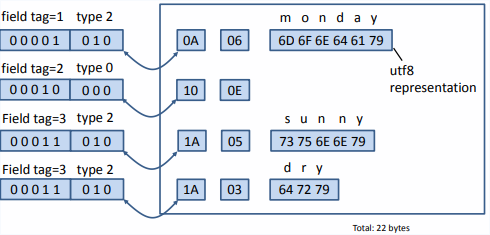
\includegraphics[width=.45\linewidth]{chap2_6.png}
\textbar \textbf{+:}efficient writing/parsing,well documented,Versioning \textbf{-:}No RPC
\rtext{ApacheThrift:framwork, applied Hadoop and HBase}
.thrift: \lstinline{struct Forecast{1: string weekday 2: i32 temperature 3: list<string> tags}\}}
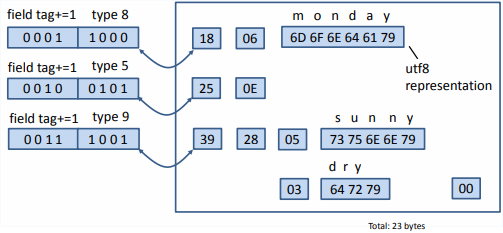
\includegraphics[width=.45\linewidth]{chap2_7.png}
\textbar \textbf{+:}Multiple protocols to serve different purposes(binary, JSON),RPC,Open source,widely,Versioning
\rtext{VariableLength:}
\section{Chap3-PRC/SessionLayer}
\rtext{Remote Procedure Call}: Call non-local procedure on remote machine, like local call
\textbar Hidden: Definition of message and content types, Marshalling/unmarshalling of parameters, Sending/receiving messages
\btext{Sequence, COMU} 
1.Client RPC, issues request to a client stub (a proxy object).
\textbar 2. Client stub encodes parameters(marshalling, Chap2)
\textbar 3. Given a network address(LAN, Internet), the client stub calls the server stub via RPC. 
The RPC can be executed using a RPC library,a socket connection or another protocol.
\textbar 4. The server stub receives the RPC.
\textbar 5. The server sub decodes the parameters(ummarshalling) and calls the local procedure on the server.
\textbar 6. Server executes RPC.
\textbar 7. Local procedure $\overset{result}{\rightarrow}$ server stub $\overset{result}{\rightarrow}$ client.
\btext{Parameter}
CallByValue: easy forRPC
\textbar CallByRef: notForRPC (client,server different address spaces) $\rightarrow$ call-by-copy (serialize objects with Thrift, Protocol
Buffers)
\btext{Binding}
StaticB: Hardcoded reference to server 
\textbar Simple and effective, no additional infrastructure
\textbar Client and Server tightly coupled
\textbar \textbar 
DynamicB:
Relies on Name and directory services to locate servers
\textbar Cost is in additional infrastructure, protocol and registration primitives
\textbar in 3. C requests service, executes RPC with S address. NameService provides S address (S registed service at directory)
\btext{RPC Sockets}in 3: RPC call, p2p comm, connect S port. S accept connection.
\btext{Error}
1.LostRequest(longer than Timeout of C,resend $\overset{SequenceNum}{\rightarrow}$ NoDuplicates)
\textbar 2.LostReply(S caches result, resend back whenDuplicates. If reply acknowledged,delete cache)
\textbar 3.ClientCrash(S waits ACK forever, orphan. 
C restart $\overset{SessionCounter}{\rightarrow}$  old reply not interfere with new requests)
\textbar 4.ServerCrash(C notKnow RPC executed or not. S logs keepingstate of the procedure $\rightarrow$ noMultiExecutions)
\btext{FailureSemantics}
1.Maybe (No repetition,Simple and efficient,No guarantee for success)
\textbar 2.AtLeastOnce(Repetition after timeout,No identification of duplicates, Acceptable for idempotent operations)
\textbar 3.AtMostOnce(Identification of duplicates:sequenceNum, No repetition, Acceptable for non-idempotent operations, No result when S crash)
\textbar 4.ExactlyOnce(State of procedure is recorded, 
Only possible with transactional processing $\rightarrow$ Atomic execution, After S crash operation can be recovered and executed exactly once)

\rtext{Remote Method Invocation RMI} Object-oriented RPC, Procedure call on remote object, Method parameters can be send two ways
(call-by-value $\rightarrow$Implement Serializable, call-by-reference $\rightarrow$ extend Remote interface),
Object reference identifies remote object
\rtext{RMIvsRPC}RPC(Procedures of remote processes are called,Service interface provides set of procedures)
\textbar RMI(Objects in different processes communicate with each other, Remote interface specifies methods of an object)
\section{C4-Naming}
\rtext{NamingService} DNS(DomainNameSystem) $\rightarrow$ url to IP of host serving this domain
\textbar A world-wide distributed database of name servers

\section{WebService}
\rtext{SOAP}Simple Object Access Protocol
Message format: Envelope(Enclosing entity of a message,Defines namespace)
Header(Contains metadata for the body,Many WS-* extensions add additional information here)
Body(Contains the payload, Further specifications define the body structure)
\rtext{RPCvsDocumentStyle}
SOAP message is constructed in a specific way, call the Web service just like a normal function, Body of message contains parameters and method name as wrapper element,marshalling/unmarshalling is part of the standard
\textbar contains no restrictions, Message body is a XML document, C/S handles the marshalling/unmarshalling
\section{Messaging\&Queuing}
\redtext{Msg Queuing Pattern}
data shared across APP diff. platforms, 
MQP transfer data frequent, immediate, reliably, 
exactly once, asy.
\redtext{Enterprise APP integration EAI}% TODO: Pub SUb
APP comm. using single Msg Bus
\\
\redtext{Msg Passing:} 
\orangetext{Msg\bluetext{=}receiver\bluetext{+}sender\bluetext{+}type\bluetext{+}payload}
\lstinline{send(message); receive(message); callback();}
\redtext{\bluetext{Messaging} vs \greentext{RMI}}
interface
\bluetext{(per Msg product) with generic operations}
\textbackslash
\greentext{required and known, but differs across apps};
\bluetext{Lower-level of abstraction than RMI}
\textbackslash
\greentext{like non-remote calls but fail potential};
\bluetext{Flexible in that messaging allows arbitrary interaction patterns between sender and receiver};
Sender \bluetext{not blocked}
\textbackslash
\greentext{blocked until reply arrives}
after sending;
\bluetext{emulate}
\textbackslash
\greentext{Realize}
request/reply pattern;
\bluetext{Asynchronous behavior hard to use debug}
\textbar \textbar \textbar
\redtext{Msg Passing Properties}
\bluetext{1.Reliability}
SequenceNum,
Ack, 
Timeout resend
$\rightarrow$Msg loss;
CheckSums, 
Error correcting codes (redundancy),
Repeat send
$\rightarrow$Msg Corruption;
Loss\redtext{+}Corruption\redtext{+}Msg encrypting
$\rightarrow$Malicious Intend
\bluetext{2.Ordering}
Msg arrive in order:
FIFO(for one sender),Causal,Total(for all sender);
\greentext{GOAL:}
All Msg delivery
\redtext{OR}
Fast incomplete Msg delivery
\bluetext{3.Syn vs. Asyn send\textbackslash receive:}
\bluetext{4.Buffering Msg $\rightarrow$ Queuing}
\greentext{Transient vs Persistent Msg:}
Msg not stored
\greentext{VS}
Msg stored lifetime of sender\&receiver 
until revoked, purged, queuing, Msg queue
\textbar
\orangetext{Blocking Send\&Receive Semantics}
\orangetext{Blocks send call until Msg arrived:}
local middleware
\greentext{\textbackslash}
remote middleware
\greentext{\textbackslash}
receiving process
\greentext{\textbackslash}
processed by receiving process;
\orangetext{Blocks receive call until:}
Msg available use non-blocking polling
\greentext{\textbackslash}
Timeout
\greentext{\textbackslash}
Msg message received
\textbar
\orangetext{Syn.Comm.}
Sender blocked until Re. done,
Receiver blocked until Se. done,
Syn equalizes Se.Re. speed
$\rightarrow$
Deadlock(both send wait),
\btext{++:}
Se. knows Msg was received,
Only one Msg buffered,
Synchronizes Se. and Re. operating diff. speeds
\btext{--:}
coupled (at same time),
blocked(deadlock, no paral.)  
\orangetext{Asy.Comm.}
Send not blocked; 
\greentext{MW buffers Msg} on Se.\textbackslash Re.,
\greentext{SenderBuffer} send faster > transmission,
\greentext{ReceiverBuffer} receive more Msg > processing,
$\rightarrow$
Buffers temporarily(not permanently) mitigate speed difference
\btext{++:}
ring buffer,
loosely coupled, not same time,
parallelism
\btext{-:}
Se. know Msg received,
Buffers overflow,
Dev. Debug. complex
\redtext{Msg Buffering}
\bluetext{send buffer full}
$\rightarrow$
Se. block,
buffered Msgover-written,
Return Exception, error
\textbar
\bluetext{receive buffer full}
$\rightarrow$
Msg dropped,
buffered Msg over-written,
return NACK to MW at Se..
\redtext{Sliding Window Protocol TCP}
prevent Re. buffer overflow:
send side may only have number of Un-ACK Msg (sliding window):
Re. send ACK,
SW size determined statically or dynamically
$\rightarrow$
size < buffer size (nooverflows),
size > buffer size(high throughput but can overflow
flow control (dynamically adjusting the window size)
\redtext{Syn Comm via Asy MW:}
Se. wait for Re. ACK
\\
%
%
%
\mysubsection{Queuing}
\greentext{Msg passing\bluetext{+}Msg buffering}
\redtext{Dequeue:}
\bluetext{Remove:}
remove Msg if dequeued
\bluetext{Browse:}
still available for other Re. if dequeued
\redtext{Decoupling Ser,Rer}
$\rightarrow$
indirect and asy comm.(asyn received via Callback = deque)
\bluetext{Space de.}Se not know Re, but know Queue,
\bluetext{Time de.}Se Re not same time,
\bluetext{Flow de.}Sending not blocked$\rightarrow$non-blocking enqueue
\redtext{Msg Queuing Pattern:}
OneToOne, OneToMany, ManyToOne, ManyToMany
\redtext{Queue Manager:}
Specialized component to queuing functionality to apps
administrative functions(create, delect, start, stop of queue)
\redtext{Multiple Consumer Queue Msg Property:}
\bluetext{Priority:}
\orangetext{Static:}
High first
\redtext{OR}
Weighted fair scheduling:\begin{CJK*}{UTF8}{gbsn}交换 a:weight2 abacabac\end{CJK*}
\orangetext{Dynamic:}
Priority change,
Earliest deadline first EDF,
Least laxity first LLF(min time left to DDL)
\bluetext{Earliest dequeue time:}
before it Msg not dequeued
\bluetext{Expiration time:}
Msg deleted if expires
\bluetext{Correlation identifier:}
match req with reply
\\
%
%
\redtext{TX Queue}
fail recovery;
\greentext{ACID atomic consistent isolated durable};
Enable local Msg TX;
commits succeeds or aborts fails;
Msg received/sent if commits;
\bluetext{Producer side}
Msg kept until commit, If aborts, Msg discarded;
\bluetext{Consumer side}
All consumed Msg kept until commit, If aborts, re-delivered;
%
\redtext{Request/Reply Queue,not atomic}
\orangetext{Req with correlationID} to match reply at C
C
\bluetext{1.Req Enque}
$\rightarrow$
Req.Que
\bluetext{2.Req.Deq}
$\rightarrow$
S
\bluetext{3.Req.process Rep.Enque}
$rightarrow$
Rep.Que
\bluetext{4.Rep.Deq}
$\rightarrow$
C
%
\redtext{Request/Reply TX Queue}
local TX:
\bluetext{1.C RequestTX:}
C enq req.
\bluetext{2.S TX:}
S deq req, processes, enq reply
\bluetext{3.C Reply TX:}
C deq. reply
\orangetext{
C RequestTX committed:
Req. process exactlyOnce,
Reply process atLeastOnce}
\bluetext{R\textbackslash R TX workaround:}
C ReqTX
\{Start enqueueRequest\bluetext{1.enq.} Commit\}
$\rightarrow$
Req.Que 
$\rightarrow$
S TX\{Start dequeueRequest\bluetext{1} enqueueReply\bluetext{2.enq.} Commit\}
$\rightarrow$
Rep.Que 
$\rightarrow$
C RepTX\{Start dequeueReply\bluetext{2} Commit\}
\textbar
\orangetext{C checks queues}
Req. in req. que.
\redtext{OR}
Req. currently processed by S
\redtext{OR}
Reply in reply que.
\orangetext{Case of Abort}
C Request TX abort, req enq. undone;
STX abort, req deq.\& reply enq undone;
C Reply TX abort, reply deq undone
\\
\redtext{\hlgray{C crash, Recovery}}
\hlgray{Persistent at C and queue manager:}
\orangetext{\hlgray{C marks req with ID,
QM store IDs of the last enqueued request $R_e$,
the last dequeued reply $R_d$, updated after commits.
$R$:ID of most recent request by the C (stored by C)}}:
\bluetext{\hlgray{1.C ReqTX not commit}}
\hlgray{
$R\neq R_e$
during TX1, resend, Empty queues, old $R_e$ in QM}
\bluetext{\hlgray{2.C ReqTX committed but S TX not$R_e=R\neq R_d$, in ReqQueue like(18,ACK)}} 
\hlgray{
Req in ReqQue(req.que.size!=0, after TX1, dequeue)}
\redtext{OR}
\hlgray{being processed by S(req.que.size=0, after TX2, C wait)}
\bluetext{\hlgray{3.S TX committed but C RepTX not}}
\hlgray{
Reply in Rep.Que(nonempty, R = $R_e$, QM's C's ReplyID un-match)},
\bluetext{\hlgray{4.C RepTX committed}}
\hlgray{
$R=R_d$
Successful,after TX3, continue}
\\
\redtext{\hlgray{Distributed TXQueuing Two-Phase Commit 2PC:}}
Only \orangetext{Atomicity},
\bluetext{\hlgray{Coordinator}}
\hlgray{among registered nodes to achieve consensus
and requests all nodes to vote;
commit, if} \orangetext{\hlgray{all}} \hlgray{voted to commit;}
\hlgray{abort, if} \orangetext{\hlgray{one}} \hlgray{voted to abort;}
\bluetext{\hlgray{1.Prepare}}
\hlgray{to commit, voting phase
Once a participant voted to commit, no longer abort the TX}
\bluetext{\hlgray{2.Commit}}
\hlgray{completion phase;}
\orangetext{\hlgray{commit, after all participants prepared
Otherwise all abort}}
\redtext{\hlgray{Sequence Diagram:}}
\bluetext{Coordinator}
$\overset{prepare}{\rightarrow}$
participant 1,2,3
$\overset{vote:commit}{\rightarrow}$
\bluetext{Coor.}
$\overset{commit}{\rightarrow}$
participants
$\overset{done}{\rightarrow}$
\bluetext{Coor.}
\textbar \textbar \textbar
\bluetext{Coor.}
$\overset{prepare}{\rightarrow}$
participant 1,2,3
$\overset{vote:abort}{\rightarrow}$
\bluetext{Coor.}
$\overset{abort}{\rightarrow}$
participants
$\overset{done}{\rightarrow}$
\bluetext{Coor.}
\redtext{\hlgray{uncertainty phase:
when p sended vote:commit until p received abort as global decision}}:
\bluetext{Uncertain part.} blocked until certain,
not to abort,
not to commit because \bluetext{global decision} may be abort,
try to contact other parti. to find certain one
(voted abort or known decision),
can only contact uncertain parti., it is blocked (comm. failure)
\redtext{\hlgray{Timeout}}
to cope with failure (lost Msg):
not requiring consultation of other:
Coor. abort TX when it timeouts in initial or wait state;
Coor. resend commit/abort to parti. when timeout to send;
Parti. aborts TX when it timeout in initial state.
\bluetext{But} when parti timeouts in prepare,
consultation required
%
%
%
%
%
\\
\redtext{\hlgray{Class C S}}
\lstinline{ChannelFactory cf=new();Producer p;Consumer c;}
\hlgray{S C init():}
\lstinline{cf.setHost("broker.tum.de");cf.queueDeclare("req\_q", Persistent);cf.queueDeclare("res\_q", Persistent);p=cf.newProducer("req\_q");c=cf.newConsumer("res\_q");//for S change p and c, C S different init()}
\redtext{\hlgray{R\textbackslash R Queue}}
\hlgray{C send(byte[] msg):}
\lstinline{p.enqueue(msg);}
\hlgray{C byte[] receive():}
\lstinline{return c.dequeue();}
\hlgray{S run():}
\lstinline{while(true){byte[] req=c.dequeue();try{Database.store(req);p.enqueue('ACK'.toBytes()) catch(e){p.enqueue('ERROR'.toBytes());}
%
%
%
\redtext{\hlgray{Correlation:}}
\hlgray{C:}
\bluetext{+}
\lstinline{Hashmap<Guid,byte[]> intermediate=new();Hashmap<Guid,Correlation>correlations=new();//two also for Broker}
\hlgray{C run():}
\lstinline{Thread.start(new Thread(){void run(){while(true){Delivery d=c.dequeue();/*statt in broker responseConsumer.dequeue();*/if(d!=null){Guid g=d.getGuid();if(intermediate.containsKey(g){Correlation cor=new(g,intermediate.get(g),d.getMessage());intermediate.remove(g);correlations.add(g,cor);/*statt in Broker: clientQueues.get(guid.getClientName()).enqueue(g,cor.toBytes());*/}
\hlgray{C send(byte[] msg):}
\lstinline{Guid g=Guid.generate();p.enqueue(g,msg);intermediate.add(g,msg);//not in Broker C}
\hlgray{S run():}
\lstinline{while(true){Delivery req=c.dequeue();try{Database.store(req);p.enqueue(req.getGuid(),"ACK".toBytes()); catch(e){p.enqueue(req.getGuid(),"ERROR".toBytes());}
%
%
%
\redtext{\hlgray{Queue with Broker:}}
\hlgray{C:}
\bluetext{+}
\lstinline{String clientName}
\hlgray{C init():}
\bluetext{+}
\lstinline{/*producer*/cf.queueDeclare('req_que_broker',Persistent);cf.queueDeclare('c_que_'+clientName,Persistent);/*consumer*/}
\hlgray{C void send(): see Correlation part above}
\hlgray{C void receive():}
\lstinline{Delivery d=c.dequeue();if(d!=null){Guid g=d.getGuid();Correlation cor=new();cor.fromBytes(d.getMessage());}
\hlgray{Broker Class:}
\bluetext{+}
\lstinline{List<String> clients=new ArrayList<>();List<String> servers=new ArrayList<>();Map<String,Producer> serverQueues=new HashMap<>();Map<String, Producer> clientQueues=new HashMap<>();Consumer requestC;Consumer responseC;//CF,Host,2 HashMap like Correlation C}
\hlgray{Broker init():}
\lstinline{clients.add("c1");servers.add("s1");/*multi add*/cf.queueDeclare("request_queue_broker",Persistent);requestConsumer=cf.newConsumer("response_queue_broker");cf.queueDeclare("response_queue_broker",Persistent);responseConsumer=cf.newConsumer("response_queue_broker");for(String s:servers)/* also for client*/String queueName="server_queue_"+s;/*clinet_q*/cf.queueDeclare(queueName,Persistent);serverQueues.put(s, cf.newProducer(queueName));//clineQueues, repeat this for loop for Client}
\hlgray{Broker run():}
\lstinline{Thread.start(new Thread(){void run(){int count = 0;while(true){Delivery d=requestConsumer.dequeue();if(d!=null){intermediate.add(d.getGuid(),d.getMessage());serverQueues.get(count\%servers.size()).enqueue(d.getGuid(),d.getMessage());count++;//HERE: REUSE Correlation: Client run() function}
\hlgray{S:}
\bluetext{+}
\lstinline{String serverName}
\hlgray{S init():}
\lstinline{/*cf.setHost*/cf.queueDeclare("resp\_q\_broker", Persistent);cf.queueDeclare("s\_q"+serverName, Persistent);p=cf.newProducer("resp\_q\_broker");c=cf.newConsumer("s\_q"+serverName);}
\hlgray{S run():}
\lstinline{while(true){Delivery d=c.dequeue(try{Database.store(request);p.enqueue(d.getGuid(),"ACK".toBytes());catch(e) p.enqueue(d.getGuid(),"ERROR".toBytes());}
%
%
%
\redtext{\hlgray{TX Queue}}
\bluetext{+}
\hlgray{C:}
\lstinline{Queue<byte[]>messageBuffer=new;Queue<Delivery>resultBuffer=new;}
\hlgray{C request():}
\lstinline{guid=Guid.generateRandom();f=newFile("path");f.write(guid);startTX message=messageBuffer.get();producer.enqueue(guid,message); commitTX}
\hlgray{C reply():}
\lstinline{startTX Delivery d=c.dequeue();resultBuffer.put(d); commitTX;}
\hlgray{C recovery():}
\lstinline{f=newFile("requestFile");Guid R=f.readLastEntry(); Guid Re=cf.getLastEnqueued("request_queue");Guid Rd=cf.getLastDequeued("reply_queue");if(R!=Re)requestTX() else if(R!=Rd){while(cf.getQueueSize("reply_queue")==0) Thread.sleep(500);/*wait all out*/ replyTX() else/*nothing*/spawn(while(true))}
\hlgray{S:}
\lstinline{processTX startTX Delivery d=c.dequeue();p.enqueue(d.getCorrId(),"ACK"); commitTX;}
\section{7QueuingTheory}
ArrivalRate$\lambda=\frac{1}{mean inter-arrival time}$
\textbar
ServiceRate $\mu=\frac{1}{mean service time}$
\textbar
Q.Formation $\equiv \lambda > \mu$
\textbar
Stability $\equiv \lambda < \mu$: busy,idle alternating
\textbar
Throughput:average \# completed jobs per unit of time $\rightarrow$ 0(stable) to maximumThr.(unstableQ.,best performance) 
\textbar
ServerUtilization $= \lambda * \mu$: S busy time percent
\textbar
A/S/n: arrival process/ service process/\# S
\textbar A,S:M (Markov,Exponential probability density),
D (Deterministic, All customers have the same value),
G (General, Any arbitrary probability distribution)
\textbar
M/M/1: Infinite population of customers, Infinite q.capacity, FIFO
\textbar
Exponential distribution: $f(x)=\lambda e^{-\lambda x}$, mean$= 1/\lambda$
\textbar
Poisson arrival process(arrivalProcess): $P_n(t) = \frac{(\lambda t)^n}{n!}e^{-\lambda t}$,
\textbar
Traffic intensity (occupancy): $\rho = \lambda/\mu$, n customers: $Prob[n] =\rho^n(1-\rho)$, empty: $Prob[n=0]=1-\rho$
\textbar
Mean \# customers: $N = \frac{\rho}{1-\rho} = \frac{\lambda}{\mu - \lambda} = L$
\textbar
Total waiting time (including service time): $T=\frac{1}{\mu - \rho}$
\section{S-Side Architecture}
\redtext{Thread:}
has own Stack, 
Instruction pointer, 
Processor State(Register). 
multiple included in proc.
\redtext{Process:}
running prog. as set of Th.
\redtext{Single‐threaded Pro.:}
One instance of virtual memory
\redtext{Multi‐threaded Pro.:}
One instance
\redtext{+}
\bluetext{th share same memory address space(obj)}
\redtext{Synchronisation:}
sharing same add.(obj), 
Read/Write access synchronized(Mutex, Locks, Semaphores)
\bluetext{Lock:}
\lstinline{Lock l; l.lock();/*critical section,can be Deadlock*/l.unlock();}
\bluetext{Mutal Exclusion:}
Critical sections of Th.s not overlap
\bluetext{Freedom from deadlock, Freedom from starvation}
%
\redtext{Th. State:}
Created
$\rightarrow$
Waiting(Scheduled or unscheduled)
$\leftrightarrow$
Swapped outWaiting(No enough memory), Running
$\rightarrow$
Terminiated, Blocked(Blocking IO)
$\rightarrow$
Waiting(IO finish)
\textbar
Blocked
$\leftrightarrow$
Swapped out andBlocked(No enough memory)
\\
\redtext{API}: 
\lstinline{public class WorkThread extends Thread{public ConnectionHandleThread(Parameter params) @Overridepublic void run(){Computation();//]}
\lstinline{/*use*/Thread t=new WorkThread(params);th.start();Thread.sleep(1000);/*current th*/th.getState();/*NEW, RUNNABLE, BLOCKED, WAITING, TERMINATED, TIMED_WAITING*/th.setPriority(para);th.yield();/*give current use of processor to other th.*/}
\\
\redtext{Amdahl Law:}
max theoretical speedup use multi processors
$T(n)=T(1)*(B+\frac{1}{n}(1-B))$
n:\# processor,
$B\in[0,1]$ is serial,nonparallizable,
speedup:$S(n)=\frac{T(1)}{T(n)}=\frac{1}{T(n)}$
\\
\redtext{Overload}:
\bluetext{1.Transient ov.}
Short spikes in req which ov. the S temporarily
\bluetext{2.Continous ov.}
Incomming exceeds S capacity
\bluetext{3.Methods to tackle ov.}
Refuse req. after certain queue length, Add capacity
\redtext{Concurrency Models}
\bluetext{1.Th‐based conc.}
One req completely handled by single th.;
single th. is responsible until response returned;
If req blocked (DB access), th. blocked
%
%
\bluetext{2.Event‐based conc.}
\redtext{not th. based}
\greentext{
Req in Network/HDD
$\rightarrow$
EventHandler
$\rightarrow$
\# FSM = \# Steps(th.s)
$\rightarrow$
Response}
\btext{--:}
Only non‐blocking(async) I/O operations used,
Code less modular, 
nonreusable,
Complex control flow(FSM, flags), debugging
OS support like async I/O libraries
\greentext{A th. processes req until th. blocked.
When th. blocked, th. continues with the next requests,
Once a th. becomes unblocked, it gets enqueued in the list of ready tasks.}
Scalar code separated in micro tasks.
\redtext{Finate State MachinesFSM:}
Java NIO to track state,
C socket created
$\rightarrow$
\bluetext{th1 accept connection}
register 'C socket event'
\textbar
requests from C socket
$\rightarrow$
\bluetext{th2 lookupDB}
register 'query done event'
\textbar
QueryDone
$\rightarrow$
\bluetext{th3 send 1MB to C}
register 'data sent event'
\textbar
data sent
$\rightarrow$
\bluetext{th4 Cancel connection} 
%
%
\\
\rtext{Single‐threaded S = Iterative S:}
S with only one worker th.
\orangetext{do all also I/O},
\bluetext{Thread‐based conc.}
\greentext{
if inout queue empty then Waits till new req from Network enqueued, 
Dequeue next req.,
single worker th. Compute req result, 
send response to Network},
\orangetext{When blocked due to I/O, th. also blocks(I/O read disk to memory)}
\btext{++:}
Simple, 
Cache Locality(one request in cache)
\btext{--:}
Insufficient use of resources, 
Limited scalability(reject requests if too many)
\rtext{Multi‐threaded S}:
S with \orangetext{multi worker th.}
\bluetext{Workaround: like above} 
as single th. wait \dots block;
OS can schedule non‐blocked th.
\orangetext{get nonblocked th. from pool};
more th. than cores since a certain percentage of I/O is assumed
\btext{++:}
\bluetext{Programming abstraction}
Divide up work to assign to th.
\bluetext{Parallelism}
throughput
\bluetext{Responsiveness}
heavy operations in back with UI still responsive
\bluetext{Blocking I/O}
If blocking I/O, other th. continue to work
\bluetext{Context switching}
Switch costs from th. to another within same process 
\orangetext{cheaper than} 
process‐to‐process switch,
\bluetext{Memory savings}
Th. to share memory, yet utilize multi units of execution
\\
\rtext{One th. per request/Connection:}
scheduled by operations,
\greentext{
Req in Network
$\rightarrow$
InputQueue
$\rightarrow$
Dispatcher
(starts a th. per req,when response sent, th. ends)
$\rightarrow$
Response to Network}
\btext{++:}
Simple 
\btext{--:}
Too many th.
$\rightarrow$
thread‐starvation(little CPU‐time),
cost to Start/Remove th., 
Not ideal for high parallel S
\lstinline{ServerSocket ss = new();ss.bind(new InetSocketAddress("127.0.0.1", port));while(true){Socket clientSocket=ss.accept();Thread t=new ConnectionHandleThread(kv,clientSocket);t.start();}
\btext{+++}
\lstinline{public class ConnectionHandleThread extends Thread{public ConnectionHandleThread(KVStore store, Socket clientSocket)/*[..]*/@Override public void run(){BufferedReader in=clientSocket.getInputStream();PrintWriter out=clientSocket.getOutputStream();String s; while((s=in.readLine())!=null){String res=kv.process(firstLine);out.write(res);out.flush();}
\\
\redtext{Abstracting Th.:}
deadlock \& starvation free
\bluetext{Abstractions:}
\greentext{Thread pool, Event based concurrency, SEDA, Actor model, Reactive programming}
\bluetext{1.Th. pool}
managed set of available th.s,
size as max(eg number of CPU cores),
do tasks in parallel,
Reuses th. for multi tasks
\orangetext{Optimal Size}
depends on \# cores, \# blocking of I/O operations
\greentext{
Request in Network
$\rightarrow$
InputQueue
$\rightarrow$
Scheduler(Thread pool with size)
$\rightarrow$
Response to Network}
\lstinline{ExecutorService es= Executors.newFixedThreadPool(4);while(true){Socket clientSocket=serverSocket.accept();es.submit(new ConnectionHandlerRunnable(kv,clientSocket));}
\bluetext{++:}
RUNNABLE above in One th. per request/Connection
\bluetext{2.Scheduling Algo:}
Most cache efficient to assign task to th.s in pool
\orangetext{Two main paradigms}:Work sharing, Work stealing
\greentext{Work Sharing Algo.:}
When th. created, scheduler moves work of other th. to new th.
\btext{--:}
Comm. between cores, Cache misses
\greentext{Work stealing algo.:}
Under-utilized processors steal work from busy processors
(The migration of threads occurs less frequently with work stealing than with work sharing)
\redtext{++:}
Maintain th. on same CPU(data locality
$\rightarrow$
better cache usage, 
Min comm. between th
%
%
\bluetext{3.Futures:}
result of asyn. computation in th. pool
\lstinline{/*result in future obj*/FutureTask<LinearRegressionResult> future=new<Integer>(new Callable<String>(){public Integer call() {List<Doubles> lr=getDailyTurnover(..);return calcLinearRegression(lr);); threadpool.execute(future);}
%
%
\bluetext{4.SEDA:}
Staged event‐driven architecture, a network of stages connected by event queues
\btext{++:}
Support massive concurrency,
Simplify the construction of services(Provide abstractions),
introspection(Adapt behavior to change load conditions),
Support self‐tuning resource managment,
Server is created from many SEDA stages
%
%
\bluetext{5.Actor:}
No access to shared memory(No locks,no deadlock), 
Scheduled on top of threads
%
%
\bluetext{6.Reactive Programming:}
oriented around data flows and propagation of change(Dependency graph)
\\
\redtext{App S:}
a component‐based product that resides in the middle‐tier of a server‐centric architecture.
It provides middleware services for security and state maintenance, 
along with data access and persistence.
\bluetext{Java:}WildFly, Websphere
\textbar
\btext{EJB}:
Standard component architecture,
Distributed business application(
(Support development, deployment and use of web services),
Write once, run in all application containers
\btext{++:}
Developer not to care Fail‐over, 
Clustering, 
(Distributed) Transaction handling, 
DB, 
Security, 
Deployment
\section{Publish/Subscribe}
\redtext{Enterprise Application Integration EAI:}
Order Entry
to
Order Scheduling
\&
Credit Validation
to
Order Release
to
Allocation
to 
Warehouse Management SY
to
Accounts Receivable
\bluetext{Required:}
Msg dissemination via bus;
De-coupled operation;
Dynamic evolution;
Location transparency;
Reliable message delivery;
Certified message delivery;
Fault tolerance;
Distributed event-based processing;
Event detection 
dissemination 
filtering 
correlation 
\redtext{Key of Pub/Sub:}
Many-to-many:
For comm.,
For coordination,
$M$: data sources (publishing C)
$n$: data sinks (subscribing C)
\greentext{+}
C \bluetext{decoupled},
not know each other
$\leftrightarrow$
\bluetext{tightly coupled Observer Design Pattern:}
No explicit dependencies, 
No coordination synchronization, 
Increase scalability of dis. SY,
Create highly dynamic(frequent add/remove) decentralized SY,
Decoupling in \orangetext{three dimensions:}
\greentext{Space Dec.}
No need for C (publishers \& subscribers) to hold references, C physically distributed,
\greentext{Time Dec.}
C not available same time(Event in Buffer)
\greentext{Syn. Dec.}
Control flow not blocked by interaction
\redtext{Decoupling in Diff. Interaction}
\begin{tabular}{c|c|c|c}
  \hline			
  Abstrac.&SpD&TD&SyD\\
  \hline
  MagPassingP2P&N&N& Producer\\
  PRC/RMI&N&N&Pro.\\
  Asy.PRC/RMI&N&N&Y\\
  FuturePRC/RMI&N&N&Y\\
  OberverPattern&N&N&Y\\
  TupleSpace&Y&Y&Pro.\\
  MsgQueue Pull&Y&Y&Pro.\\
  Pub/Sub&Y&Y&Y\\
  \hline
\end{tabular}
\redtext{Pub/Sub Models:}
ContentBased, 
ChannelBased(fixed, nonhierarchical), 
TopicBased(SubjectBase, hierarchical, sport news USA)
\redtext{Matching\&Filtering Content-based:}
event(Publication) $e$, 
set of subscriptions $S$, 
find all subs. $s\in S$ match $e$.
\bluetext{Subscription:}
Boolean func over predicates
\bluetext{Publication(event):}
Sets of attribute-value pairs
\\
\rtext{Two-phased Matching Algo.}
1.Match all predicates 
\bluetext{Predicate Matching Phase}
2.Match subscri. on last Phase 
\bluetext{Subscriptions Matching Phase}
\redtext{1.Predicate Mat.P.:}
set $P$ of predicates, 
event $e$, 
identify all true pred. $p$ of $P$
$\rightarrow$
\orangetext{Predicate bit vector},
Hash key: attribute name
\bluetext{General Purpose Data Structure:}
for single attr.:
4 ordered linked list(b tree) for
$=, <, >, !=$
operators,
$O(n)$ all events\&lists
\bluetext{Finite Predicate Value Domain Types:}
big matrix \greentext{eg 1000*4 for Price$\in$[1, 1000],
1000 for price, 4 for operators}, entry lookup $m[i][j]=O(1)$
\redtext{2.Subscription Mat.P.: Counting Algo}
\greentext{
S1:A<6\&B==6, S2:A<6\&B==1
$\rightarrow$
p1:A<6,p2:B==6,p3:B==1
$\rightarrow$
pred. vector:p1(S1,S2),p2(S1),p3(S2)
come Event(A,5),(B,6)
$\rightarrow$
S1 in p1,p2 matched \#=2=\#pred. of S1}
Data Structure:
pred. vector,
bit matrix.
list
\redtext{Propagation Algo:}
Match with other pred. base on Cluster.
\greentext{Same as above,
bit vector 110 for p1,p2,p3;
Cluster:S1,S2 with p1,p2,p3
but p3 not matched, delete s2}
\\
\rtext{\hlgray{Content-based Routing}}
\bluetext{\hlgray{1.Advertisements}}
\hlgray{schema or types,data sources} 
\redtext{\hlgray{Boradcast}},
\bluetext{\hlgray{2.Publications\&events}}
\hlgray{data sources}
\begin{CJK*}{UTF8}{gbsn}
\redtext{根据上一步Broker's Subscription走}
\end{CJK*},
\redtext{\hlgray{if s1 subscribers [p,>,120],[t,>,20]=[p,>,120]$\wedge$[t,>,20]}}
\bluetext{\hlgray{3.Subscriptions}}
\hlgray{query, data sinks: if empty$\{\emptyset\}\rightarrow\emptyset$}
\redtext{\hlgray{if p1 publish [p,120],[t,20] =[p,120]$\vee + $[t,20]}}
\bluetext{\hlgray{Composite Subscription:}}
\hlgray{event correlation, in network filtering,
detection of composite events}
\begin{CJK*}{UTF8}{gbsn}
\redtext{Cached 但是只能用一次, Routing Table里面不能带OR AND 必须拆开写}
\end{CJK*}
\redtext{\hlgray{Topic Based Routing:}}
\bluetext{\hlgray{Publisher:}}
\hlgray{[l1,=,business][l2,=,*][l3,=,*][n,=,*]}
\bluetext{\hlgray{Subscriber:}}
\hlgray{[l1,=,business][l2,=,market][l3,=,stocks], 
[l1,=,business]}
\bluetext{\hlgray{Publishment:}}
\hlgray{[l1,business][l2,null][l3,null][n,n1]}

\section{Service Orchestration}
\rtext{Business Process:}
set of linked activities which realise business goal
\bluetext{Bus. Pro.} \redtext{vs} \greentext{Programs}
Granularity(Based on \bluetext{activities} \greentext{instructions}, 
Programming in \bluetext{large} \greentext{small}),
Control flow(\bluetext{Explicitly} \greentext{Implicitly} defined, 
\bluetext{Easy} \greentext{Not easy} understand),
\bluetext{Flexibility(change)},
\greentext{No Flexibility(Hard-coded)},
Execution(\bluetext{call third-party webservices}
\greentext{Invoke instructions locally},
, Scheduled by \bluetext{process engine} \greentext{OS})
%
\\
\rtext{BPEL, WS-BPEL:}
Web Services Business Process Execution Language(XML based),
to \orangetext{orchestrate loosely coupled services}
to model \bluetext{SOA's Business processe},
Def of business processes using web services at bus. proc. execution engine (ODE),
\orangetext{Lacks possibility} for formal verification compared to \greentext{FSP}
\redtext{Components:}
Activities,
State handling,
Control structures,
Exception handling,
Partner links,
Parallism,
Dead path elimination
\redtext{Related Standards:}
\bluetext{SOAP}
Simple Object Access Protocol,
Comm. platform in XML
\bluetext{WSDL}
Web Service Definition Language,
set of endpoints operating on Msg,
Operations and Msg described abstract, 
bound to concrete network protocol
\bluetext{UDDI}
Universal Description, Discovery and Integration,
Services registered, published, reused by other organizations,
App store for webservices
\\
\rtext{Service-Oriented Architecture SOA}
technique involving interaction between loosely coupled services 
that function independent;
modeled by \bluetext{WS-BPEL}.
\redtext{Principles:}
Loose coupling,
Service contract
$\rightarrow$
WSDL,
Abstraction of underlying logic,
Autonomy,
Reusability,
Composability $\rightarrow$ WS-BPEL,
Interoperability,
Discoverability $\rightarrow$ UDDI
\btext{BPMN vs BPEL}
Business friendly,
intuitive,
process oriented,
Swimlanes that represent organizational units,
User friendly data manipulations,
include human tasks,
expose web service UI
\redtext{VS}
technical,
manipulated with XPath expressions,
xpress orchestrations,
error handling,
compensating actions
\\
\redtext{Service composition}
\bluetext{conceptual model:}
S exchang Msg via out-port, in-port.
\bluetext{design methodology:}
\redtext{1Bottom-up:}
Serv. providers develop\& publish serv.;
Serv. consumers discover\&select serv.;
Serv. consumers compose selected serv..
\redtext{2Top-down:}
Serv. consumer develop global process;
Serv. consumers decompose global process into subprocess;
Serv. consumers select/develop services to implement subprocess.
\\
\redtext{Service orchestration}
\bluetext{Local perspective},
Describe control from one party‘s behavior(perspective),
\bluetext{WS-BPEL} as Standard,
Executable process which interact(Msg level) with web serv.
(Service internal / external),
Business process(business logic$+$task execution order,
span multiple apps and organizations,
Define long-lived TX multistep process model)
\\
\redtext{Service choreography}
Global perspective,
Describe global interactions among all the parties,
\bluetext{WS-CDL} as Standard
Tracks Msg sequences among multiple source and sinks,
Each involved party describes its part of the interaction
\bluetext{Orchest. vs Choreo.}
Two Orchest.(Web Service) sending each other(Choreo.)
\bluetext{Request, ACK, Accept, ACK}
\\
\rtext{Formal Methods:}
Modeling approaches, State machine verification,
(Finite state processes FSP, BPEL $\rightarrow$ LTS $\rightarrow$ FSP),
to represent and reason about \bluetext{Complexity of Concurrency Sy},
Performance optimization,
Deadlock detection, 
Dead Path elimination
\rtext{FSP}
Labeled Transition SY(
Abstract machine to study computation
Contains set of states and transitions between states)
\\
\bluetext{1.BPEL Basic Activitiy:
Receive,
Invoke,
Reply,
Assign,
Throw,
Exit,
Wait,
Empty.}:
Variable:
Global visibility <process>;
Visibility only within a <scope>.
<variables>
<variable name="coursename" type="xsd:string"/>
<variable name="grade" type="myNS:typeFromAnotherWSDL"/>
</variables>
\bluetext{2.BPEL Structured Activitiy:
Sequence,
If,
While Loop,
repeatUntil,
forEach,
Pick(Specifies which process executed check received event),
Flow,
Scop(exception).}
<while>
<condition>
\$iterations \&lt;3
</condition>
<invoke name="callSomeWebservice" ... />
</while>
\redtext{OR}
<forEach parallel="yes"counterName="N">
<startCounterValue>1</startCounterValue>
<finalCounterValue>5</finalCounterValue>
<scope>
<invoke name="callSomeWebservice"/>
</scope>
</forEach>
\rtext{BPEL$\rightarrow$FSP}
<invoke partner='p1' operation='o1'/>$\rightarrow$INVOKE = (invoke\_p1\_o1->END).
<receive partner='p2' operation='o2'/>$\rightarrow$RECEIVE = (receive\_p2\_o2->END).
<reply partner='p1' operation='o1'/>$\rightarrow$REPLY = (reply\_p1\_o->END).
\bluetext{Sequence}:
<sequence>
\begin{CJK*}{UTF8}{gbsn}
  \redtext{见上面BPEL三个}
\end{CJK*}
</sequence> 
$\rightarrow$
\begin{CJK*}{UTF8}{gbsn}
\redtext{见上面FSP三个}
\end{CJK*}
SEQUENCE = INVOKE; RECEIVE; REPLY; END. 
$0 \rightarrow 1\rightarrow 2 \rightarrow E$
\bluetext{Flow: Parallel Activity}
<flow>
\begin{CJK*}{UTF8}{gbsn}
\redtext{见上面BPEL三个}
\end{CJK*}
</flow>
$\rightarrow$
\begin{CJK*}{UTF8}{gbsn}
\redtext{见上面FSP三个}
\end{CJK*}
|| FLOW = (INVOKE || RECEIVE || REPLY).
$0 \rightarrow 1\rightarrow 2 \rightarrow E \leftarrow 4 \leftarrow 5 \leftarrow 6 \leftarrow 7$
\begin{CJK*}{UTF8}{gbsn}
\redtext{而且每点出3种Activity}
\end{CJK*}
\textbar
\rtext{\hlgray{Deadlock Detection}}:
\hlgray{when two or more competing activities are each waiting for the other to finish,}
\redtext{\hlgray{in FSP: a non-final-state with no outgoing arcs, like A sends to B, B sends to A}}
\bluetext{\hlgray{Assumption: Sync Comm}}
\hlgray{$!m_1$: Send a Msg of type m,
$?m_1$: Receive a Msg of type m}
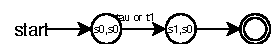
\includegraphics[width=\linewidth]{Deadlock_FSM.pdf}
\hlgray{$\tau$ for merge step}
\end{multicols*}
\end{document}
